\documentclass{ximera}

% MATH -----------------------------------------------------------
\newcommand{\nats}{\mathbb N}
\newcommand{\ints}{\mathbb Z}
\newcommand{\rats}{\mathbb Q}
\newcommand{\reals}{\mathbb R}
\newcommand{\complex}{\mathbb C}
\newcommand{\powerset}{\mathscr P}

%-------------------------------------------------------------

\pgfplotsset{compat=1.18}
\begin{document}
\begin{abstract}
 \end{abstract}

    \title{Exemplar Examples 6}
    
    \maketitle

Here is part of an approximate direction field for the first order differential equation $(4y^3-x)y^{\,\prime}=y-2x$.

% x^2-xy+y^4=1  


\begin{figure}[h]
\centering
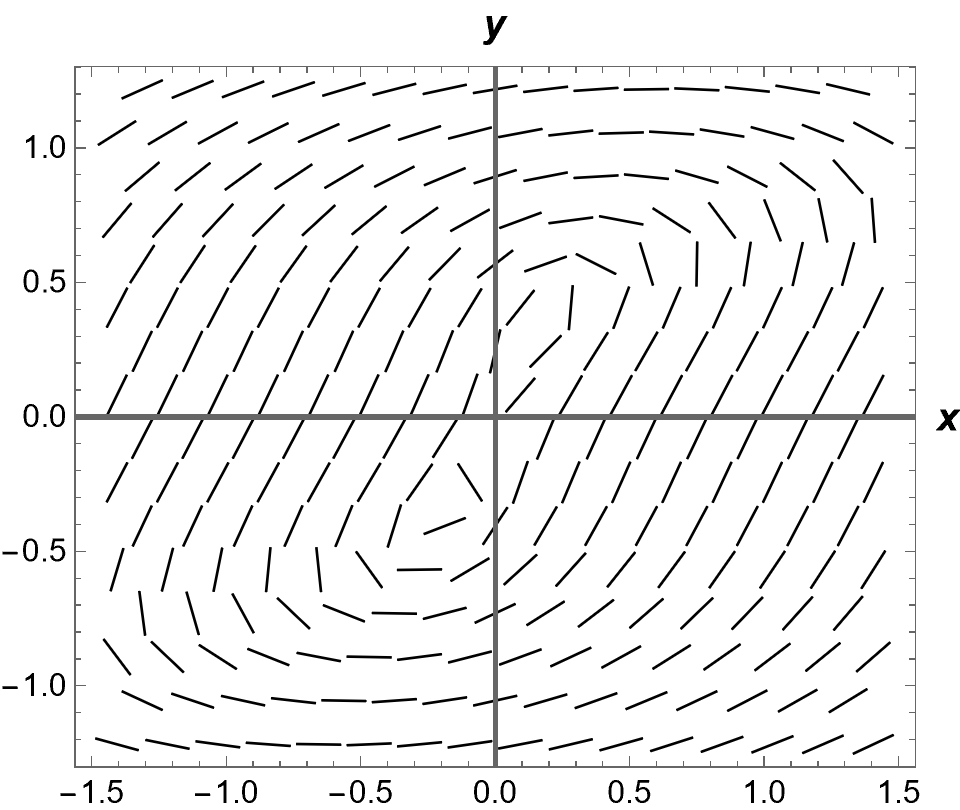
\includegraphics[scale=0.8,alt={A direction field.}]{ExemplarSixDirectionField.png}
\caption{A direction field}
\end{figure}

\begin{enumerate}

\item Let's draw the integral curve in the direction field passing through $(-1,0)$.  

\item Is this differential equation linear?  Separable?  Bernoulli?  Nonlinear homogeneous?    

\item Let's rewrite this equation in the form $M\,dx+N\,dy=0$.

% (2x-y) dx+ (4y^3-x) dy=0

\vfill


\item Let's check for exactness. 

\vspace{2cm}

\newpage

\item Let's solve this equation for an implicit general solution.

% x^2-xy+y^4=C

\vfill


\item Suppose $y(x)$ satisfies $(4y^3-x)y^{\,\prime}=y-2x$, $y(-1)=0$.  Let's find the solution(s) to $y(x)=1$.

% x^2-xy+y^4=1

% x^2-x+1=1---> x=0 or x=1.


\vfill

\end{enumerate}


\end{document}